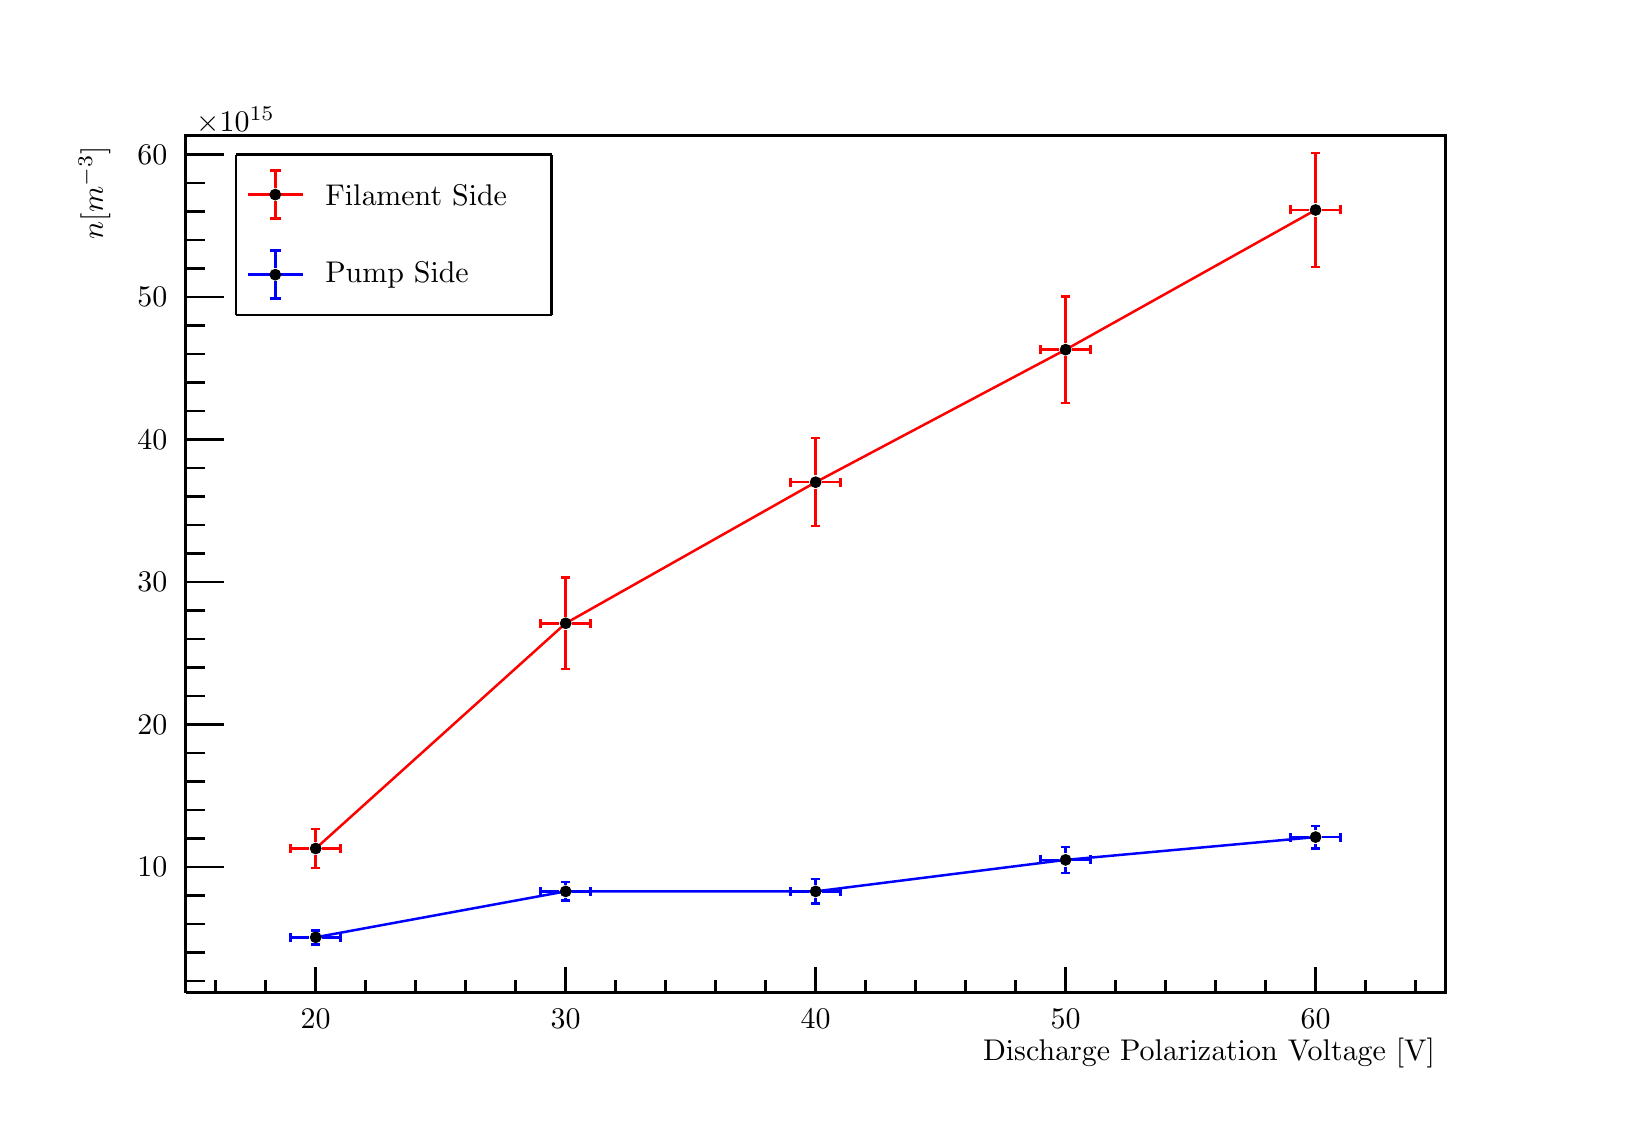
\begin{tikzpicture}
\pgfdeclareplotmark{cross} {
\pgfpathmoveto{\pgfpoint{-0.3\pgfplotmarksize}{\pgfplotmarksize}}
\pgfpathlineto{\pgfpoint{+0.3\pgfplotmarksize}{\pgfplotmarksize}}
\pgfpathlineto{\pgfpoint{+0.3\pgfplotmarksize}{0.3\pgfplotmarksize}}
\pgfpathlineto{\pgfpoint{+1\pgfplotmarksize}{0.3\pgfplotmarksize}}
\pgfpathlineto{\pgfpoint{+1\pgfplotmarksize}{-0.3\pgfplotmarksize}}
\pgfpathlineto{\pgfpoint{+0.3\pgfplotmarksize}{-0.3\pgfplotmarksize}}
\pgfpathlineto{\pgfpoint{+0.3\pgfplotmarksize}{-1.\pgfplotmarksize}}
\pgfpathlineto{\pgfpoint{-0.3\pgfplotmarksize}{-1.\pgfplotmarksize}}
\pgfpathlineto{\pgfpoint{-0.3\pgfplotmarksize}{-0.3\pgfplotmarksize}}
\pgfpathlineto{\pgfpoint{-1.\pgfplotmarksize}{-0.3\pgfplotmarksize}}
\pgfpathlineto{\pgfpoint{-1.\pgfplotmarksize}{0.3\pgfplotmarksize}}
\pgfpathlineto{\pgfpoint{-0.3\pgfplotmarksize}{0.3\pgfplotmarksize}}
\pgfpathclose
\pgfusepathqstroke
}
\pgfdeclareplotmark{cross*} {
\pgfpathmoveto{\pgfpoint{-0.3\pgfplotmarksize}{\pgfplotmarksize}}
\pgfpathlineto{\pgfpoint{+0.3\pgfplotmarksize}{\pgfplotmarksize}}
\pgfpathlineto{\pgfpoint{+0.3\pgfplotmarksize}{0.3\pgfplotmarksize}}
\pgfpathlineto{\pgfpoint{+1\pgfplotmarksize}{0.3\pgfplotmarksize}}
\pgfpathlineto{\pgfpoint{+1\pgfplotmarksize}{-0.3\pgfplotmarksize}}
\pgfpathlineto{\pgfpoint{+0.3\pgfplotmarksize}{-0.3\pgfplotmarksize}}
\pgfpathlineto{\pgfpoint{+0.3\pgfplotmarksize}{-1.\pgfplotmarksize}}
\pgfpathlineto{\pgfpoint{-0.3\pgfplotmarksize}{-1.\pgfplotmarksize}}
\pgfpathlineto{\pgfpoint{-0.3\pgfplotmarksize}{-0.3\pgfplotmarksize}}
\pgfpathlineto{\pgfpoint{-1.\pgfplotmarksize}{-0.3\pgfplotmarksize}}
\pgfpathlineto{\pgfpoint{-1.\pgfplotmarksize}{0.3\pgfplotmarksize}}
\pgfpathlineto{\pgfpoint{-0.3\pgfplotmarksize}{0.3\pgfplotmarksize}}
\pgfpathclose
\pgfusepathqfillstroke
}
\pgfdeclareplotmark{newstar} {
\pgfpathmoveto{\pgfqpoint{0pt}{\pgfplotmarksize}}
\pgfpathlineto{\pgfqpointpolar{44}{0.5\pgfplotmarksize}}
\pgfpathlineto{\pgfqpointpolar{18}{\pgfplotmarksize}}
\pgfpathlineto{\pgfqpointpolar{-20}{0.5\pgfplotmarksize}}
\pgfpathlineto{\pgfqpointpolar{-54}{\pgfplotmarksize}}
\pgfpathlineto{\pgfqpointpolar{-90}{0.5\pgfplotmarksize}}
\pgfpathlineto{\pgfqpointpolar{234}{\pgfplotmarksize}}
\pgfpathlineto{\pgfqpointpolar{198}{0.5\pgfplotmarksize}}
\pgfpathlineto{\pgfqpointpolar{162}{\pgfplotmarksize}}
\pgfpathlineto{\pgfqpointpolar{134}{0.5\pgfplotmarksize}}
\pgfpathclose
\pgfusepathqstroke
}
\pgfdeclareplotmark{newstar*} {
\pgfpathmoveto{\pgfqpoint{0pt}{\pgfplotmarksize}}
\pgfpathlineto{\pgfqpointpolar{44}{0.5\pgfplotmarksize}}
\pgfpathlineto{\pgfqpointpolar{18}{\pgfplotmarksize}}
\pgfpathlineto{\pgfqpointpolar{-20}{0.5\pgfplotmarksize}}
\pgfpathlineto{\pgfqpointpolar{-54}{\pgfplotmarksize}}
\pgfpathlineto{\pgfqpointpolar{-90}{0.5\pgfplotmarksize}}
\pgfpathlineto{\pgfqpointpolar{234}{\pgfplotmarksize}}
\pgfpathlineto{\pgfqpointpolar{198}{0.5\pgfplotmarksize}}
\pgfpathlineto{\pgfqpointpolar{162}{\pgfplotmarksize}}
\pgfpathlineto{\pgfqpointpolar{134}{0.5\pgfplotmarksize}}
\pgfpathclose
\pgfusepathqfillstroke
}
\definecolor{c}{rgb}{1,1,1};
\draw [color=c, fill=c] (0,0) rectangle (20,13.6103);
\draw [color=c, fill=c] (2,1.36103) rectangle (18,12.2493);
\definecolor{c}{rgb}{0,0,0};
\draw [c,line width=0.9] (2,1.36103) -- (2,12.2493) -- (18,12.2493) -- (18,1.36103) -- (2,1.36103);
\definecolor{c}{rgb}{1,1,1};
\draw [color=c, fill=c] (2,1.36103) rectangle (18,12.2493);
\definecolor{c}{rgb}{0,0,0};
\draw [c,line width=0.9] (2,1.36103) -- (2,12.2493) -- (18,12.2493) -- (18,1.36103) -- (2,1.36103);
\draw [c,line width=0.9] (2,1.36103) -- (18,1.36103);
\draw [c,line width=0.9] (3.65079,1.68768) -- (3.65079,1.36103);
\draw [c,line width=0.9] (4.28571,1.52436) -- (4.28571,1.36103);
\draw [c,line width=0.9] (4.92064,1.52436) -- (4.92064,1.36103);
\draw [c,line width=0.9] (5.55556,1.52436) -- (5.55556,1.36103);
\draw [c,line width=0.9] (6.19048,1.52436) -- (6.19048,1.36103);
\draw [c,line width=0.9] (6.8254,1.68768) -- (6.8254,1.36103);
\draw [c,line width=0.9] (7.46032,1.52436) -- (7.46032,1.36103);
\draw [c,line width=0.9] (8.09524,1.52436) -- (8.09524,1.36103);
\draw [c,line width=0.9] (8.73016,1.52436) -- (8.73016,1.36103);
\draw [c,line width=0.9] (9.36508,1.52436) -- (9.36508,1.36103);
\draw [c,line width=0.9] (10,1.68768) -- (10,1.36103);
\draw [c,line width=0.9] (10.6349,1.52436) -- (10.6349,1.36103);
\draw [c,line width=0.9] (11.2698,1.52436) -- (11.2698,1.36103);
\draw [c,line width=0.9] (11.9048,1.52436) -- (11.9048,1.36103);
\draw [c,line width=0.9] (12.5397,1.52436) -- (12.5397,1.36103);
\draw [c,line width=0.9] (13.1746,1.68768) -- (13.1746,1.36103);
\draw [c,line width=0.9] (13.8095,1.52436) -- (13.8095,1.36103);
\draw [c,line width=0.9] (14.4444,1.52436) -- (14.4444,1.36103);
\draw [c,line width=0.9] (15.0794,1.52436) -- (15.0794,1.36103);
\draw [c,line width=0.9] (15.7143,1.52436) -- (15.7143,1.36103);
\draw [c,line width=0.9] (16.3492,1.68768) -- (16.3492,1.36103);
\draw [c,line width=0.9] (3.65079,1.68768) -- (3.65079,1.36103);
\draw [c,line width=0.9] (3.01587,1.52436) -- (3.01587,1.36103);
\draw [c,line width=0.9] (2.38095,1.52436) -- (2.38095,1.36103);
\draw [c,line width=0.9] (16.3492,1.68768) -- (16.3492,1.36103);
\draw [c,line width=0.9] (16.9841,1.52436) -- (16.9841,1.36103);
\draw [c,line width=0.9] (17.619,1.52436) -- (17.619,1.36103);
\draw [anchor=base] (3.65079,0.911891) node[scale=1.08185, color=c, rotate=0]{20};
\draw [anchor=base] (6.8254,0.911891) node[scale=1.08185, color=c, rotate=0]{30};
\draw [anchor=base] (10,0.911891) node[scale=1.08185, color=c, rotate=0]{40};
\draw [anchor=base] (13.1746,0.911891) node[scale=1.08185, color=c, rotate=0]{50};
\draw [anchor=base] (16.3492,0.911891) node[scale=1.08185, color=c, rotate=0]{60};
\draw [anchor= east] (18,0.598854) node[scale=1.08185, color=c, rotate=0]{Discharge Polarization Voltage [V]};
\draw [c,line width=0.9] (2,1.36103) -- (2,12.2493);
\draw [c,line width=0.9] (2.48,2.95761) -- (2,2.95761);
\draw [c,line width=0.9] (2.24,3.31962) -- (2,3.31962);
\draw [c,line width=0.9] (2.24,3.68163) -- (2,3.68163);
\draw [c,line width=0.9] (2.24,4.04364) -- (2,4.04364);
\draw [c,line width=0.9] (2.24,4.40565) -- (2,4.40565);
\draw [c,line width=0.9] (2.48,4.76766) -- (2,4.76766);
\draw [c,line width=0.9] (2.24,5.12966) -- (2,5.12966);
\draw [c,line width=0.9] (2.24,5.49167) -- (2,5.49167);
\draw [c,line width=0.9] (2.24,5.85368) -- (2,5.85368);
\draw [c,line width=0.9] (2.24,6.21569) -- (2,6.21569);
\draw [c,line width=0.9] (2.48,6.5777) -- (2,6.5777);
\draw [c,line width=0.9] (2.24,6.9397) -- (2,6.9397);
\draw [c,line width=0.9] (2.24,7.30171) -- (2,7.30171);
\draw [c,line width=0.9] (2.24,7.66372) -- (2,7.66372);
\draw [c,line width=0.9] (2.24,8.02573) -- (2,8.02573);
\draw [c,line width=0.9] (2.48,8.38774) -- (2,8.38774);
\draw [c,line width=0.9] (2.24,8.74975) -- (2,8.74975);
\draw [c,line width=0.9] (2.24,9.11175) -- (2,9.11175);
\draw [c,line width=0.9] (2.24,9.47376) -- (2,9.47376);
\draw [c,line width=0.9] (2.24,9.83577) -- (2,9.83577);
\draw [c,line width=0.9] (2.48,10.1978) -- (2,10.1978);
\draw [c,line width=0.9] (2.24,10.5598) -- (2,10.5598);
\draw [c,line width=0.9] (2.24,10.9218) -- (2,10.9218);
\draw [c,line width=0.9] (2.24,11.2838) -- (2,11.2838);
\draw [c,line width=0.9] (2.24,11.6458) -- (2,11.6458);
\draw [c,line width=0.9] (2.48,12.0078) -- (2,12.0078);
\draw [c,line width=0.9] (2.48,2.95761) -- (2,2.95761);
\draw [c,line width=0.9] (2.24,2.59561) -- (2,2.59561);
\draw [c,line width=0.9] (2.24,2.2336) -- (2,2.2336);
\draw [c,line width=0.9] (2.24,1.87159) -- (2,1.87159);
\draw [c,line width=0.9] (2.24,1.50958) -- (2,1.50958);
\draw [c,line width=0.9] (2.48,12.0078) -- (2,12.0078);
\draw [anchor= east] (1.9,2.95761) node[scale=1.08185, color=c, rotate=0]{10};
\draw [anchor= east] (1.9,4.76766) node[scale=1.08185, color=c, rotate=0]{20};
\draw [anchor= east] (1.9,6.5777) node[scale=1.08185, color=c, rotate=0]{30};
\draw [anchor= east] (1.9,8.38774) node[scale=1.08185, color=c, rotate=0]{40};
\draw [anchor= east] (1.9,10.1978) node[scale=1.08185, color=c, rotate=0]{50};
\draw [anchor= east] (1.9,12.0078) node[scale=1.08185, color=c, rotate=0]{60};
\draw [anchor=base west] (2,12.2969) node[scale=1.08185, color=c, rotate=0]{$\times10^{15}$};
\draw [anchor= east] (0.841547,12.2493) node[scale=1.08185, color=c, rotate=90]{$n [m^{-3}]$};
\definecolor{c}{rgb}{1,0,0};
\draw [c,line width=0.9] (3.65079,3.19292) -- (6.8254,6.05278) -- (10,7.84472) -- (13.1746,9.52806) -- (16.3492,11.3019);
\definecolor{c}{rgb}{0,0,0};
\foreach \P in {(3.65079,3.19292), (6.8254,6.05278), (10,7.84472), (13.1746,9.52806), (16.3492,11.3019)}{\draw[mark options={color=c,fill=c},mark size=1.921922pt,mark=*] plot coordinates {\P};}
\definecolor{c}{rgb}{1,0,0};
\draw [c,line width=0.9] (3.56483,3.19292) -- (3.33333,3.19292);
\draw [c,line width=0.9] (3.33333,3.13561) -- (3.33333,3.25023);
\draw [c,line width=0.9] (3.73675,3.19292) -- (3.96825,3.19292);
\draw [c,line width=0.9] (3.96825,3.13561) -- (3.96825,3.25023);
\draw [c,line width=0.9] (3.65079,3.27888) -- (3.65079,3.43909);
\draw [c,line width=0.9] (3.59349,3.43909) -- (3.7081,3.43909);
\draw [c,line width=0.9] (3.65079,3.10696) -- (3.65079,2.94675);
\draw [c,line width=0.9] (3.59349,2.94675) -- (3.7081,2.94675);
\draw [c,line width=0.9] (6.73944,6.05278) -- (6.50794,6.05278);
\draw [c,line width=0.9] (6.50794,5.99548) -- (6.50794,6.11009);
\draw [c,line width=0.9] (6.91136,6.05278) -- (7.14286,6.05278);
\draw [c,line width=0.9] (7.14286,5.99548) -- (7.14286,6.11009);
\draw [c,line width=0.9] (6.8254,6.13874) -- (6.8254,6.63562);
\draw [c,line width=0.9] (6.76809,6.63562) -- (6.8827,6.63562);
\draw [c,line width=0.9] (6.8254,5.96682) -- (6.8254,5.46995);
\draw [c,line width=0.9] (6.76809,5.46995) -- (6.8827,5.46995);
\draw [c,line width=0.9] (9.91404,7.84472) -- (9.68254,7.84472);
\draw [c,line width=0.9] (9.68254,7.78742) -- (9.68254,7.90203);
\draw [c,line width=0.9] (10.086,7.84472) -- (10.3175,7.84472);
\draw [c,line width=0.9] (10.3175,7.78742) -- (10.3175,7.90203);
\draw [c,line width=0.9] (10,7.93068) -- (10,8.40403);
\draw [c,line width=0.9] (9.94269,8.40403) -- (10.0573,8.40403);
\draw [c,line width=0.9] (10,7.75876) -- (10,7.28542);
\draw [c,line width=0.9] (9.94269,7.28542) -- (10.0573,7.28542);
\draw [c,line width=0.9] (13.0886,9.52806) -- (12.8571,9.52806);
\draw [c,line width=0.9] (12.8571,9.47076) -- (12.8571,9.58537);
\draw [c,line width=0.9] (13.2606,9.52806) -- (13.4921,9.52806);
\draw [c,line width=0.9] (13.4921,9.47076) -- (13.4921,9.58537);
\draw [c,line width=0.9] (13.1746,9.61402) -- (13.1746,10.205);
\draw [c,line width=0.9] (13.1173,10.205) -- (13.2319,10.205);
\draw [c,line width=0.9] (13.1746,9.4421) -- (13.1746,8.85111);
\draw [c,line width=0.9] (13.1173,8.85111) -- (13.2319,8.85111);
\draw [c,line width=0.9] (16.2632,11.3019) -- (16.0317,11.3019);
\draw [c,line width=0.9] (16.0317,11.2446) -- (16.0317,11.3592);
\draw [c,line width=0.9] (16.4352,11.3019) -- (16.6667,11.3019);
\draw [c,line width=0.9] (16.6667,11.2446) -- (16.6667,11.3592);
\draw [c,line width=0.9] (16.3492,11.3879) -- (16.3492,12.0241);
\draw [c,line width=0.9] (16.2919,12.0241) -- (16.4065,12.0241);
\draw [c,line width=0.9] (16.3492,11.2159) -- (16.3492,10.5797);
\draw [c,line width=0.9] (16.2919,10.5797) -- (16.4065,10.5797);
\definecolor{c}{rgb}{0,0,1};
\draw [c,line width=0.9] (3.56483,2.06526) -- (3.33333,2.06526);
\draw [c,line width=0.9] (3.33333,2.00796) -- (3.33333,2.12257);
\draw [c,line width=0.9] (3.73675,2.06526) -- (3.96825,2.06526);
\draw [c,line width=0.9] (3.96825,2.00796) -- (3.96825,2.12257);
\draw [c,line width=0.9] (3.65079,2.15122) -- (3.65079,2.1545);
\draw [c,line width=0.9] (3.59349,2.1545) -- (3.7081,2.1545);
\draw [c,line width=0.9] (3.65079,1.97931) -- (3.65079,1.97603);
\draw [c,line width=0.9] (3.59349,1.97603) -- (3.7081,1.97603);
\draw [c,line width=0.9] (6.73944,2.6481) -- (6.50794,2.6481);
\draw [c,line width=0.9] (6.50794,2.59079) -- (6.50794,2.7054);
\draw [c,line width=0.9] (6.91136,2.6481) -- (7.14286,2.6481);
\draw [c,line width=0.9] (7.14286,2.59079) -- (7.14286,2.7054);
\draw [c,line width=0.9] (6.8254,2.73406) -- (6.8254,2.76503);
\draw [c,line width=0.9] (6.76809,2.76503) -- (6.8827,2.76503);
\draw [c,line width=0.9] (6.8254,2.56214) -- (6.8254,2.53117);
\draw [c,line width=0.9] (6.76809,2.53117) -- (6.8827,2.53117);
\draw [c,line width=0.9] (9.91404,2.6481) -- (9.68254,2.6481);
\draw [c,line width=0.9] (9.68254,2.59079) -- (9.68254,2.7054);
\draw [c,line width=0.9] (10.086,2.6481) -- (10.3175,2.6481);
\draw [c,line width=0.9] (10.3175,2.59079) -- (10.3175,2.7054);
\draw [c,line width=0.9] (10,2.73406) -- (10,2.80485);
\draw [c,line width=0.9] (9.94269,2.80485) -- (10.0573,2.80485);
\draw [c,line width=0.9] (10,2.56214) -- (10,2.49135);
\draw [c,line width=0.9] (9.94269,2.49135) -- (10.0573,2.49135);
\draw [c,line width=0.9] (13.0886,3.04812) -- (12.8571,3.04812);
\draw [c,line width=0.9] (12.8571,2.99081) -- (12.8571,3.10542);
\draw [c,line width=0.9] (13.2606,3.04812) -- (13.4921,3.04812);
\draw [c,line width=0.9] (13.4921,2.99081) -- (13.4921,3.10542);
\draw [c,line width=0.9] (13.1746,3.13408) -- (13.1746,3.21446);
\draw [c,line width=0.9] (13.1173,3.21446) -- (13.2319,3.21446);
\draw [c,line width=0.9] (13.1746,2.96216) -- (13.1746,2.88177);
\draw [c,line width=0.9] (13.1173,2.88177) -- (13.2319,2.88177);
\draw [c,line width=0.9] (16.2632,3.33772) -- (16.0317,3.33772);
\draw [c,line width=0.9] (16.0317,3.28042) -- (16.0317,3.39503);
\draw [c,line width=0.9] (16.4352,3.33772) -- (16.6667,3.33772);
\draw [c,line width=0.9] (16.6667,3.28042) -- (16.6667,3.39503);
\draw [c,line width=0.9] (16.3492,3.42368) -- (16.3492,3.48126);
\draw [c,line width=0.9] (16.2919,3.48126) -- (16.4065,3.48126);
\draw [c,line width=0.9] (16.3492,3.25176) -- (16.3492,3.19419);
\draw [c,line width=0.9] (16.2919,3.19419) -- (16.4065,3.19419);
\draw [c,line width=0.9] (3.65079,2.06526) -- (6.8254,2.6481) -- (10,2.6481) -- (13.1746,3.04812) -- (16.3492,3.33772);
\definecolor{c}{rgb}{0,0,0};
\foreach \P in {(3.65079,2.06526), (6.8254,2.6481), (10,2.6481), (13.1746,3.04812), (16.3492,3.33772)}{\draw[mark options={color=c,fill=c},mark size=1.921922pt,mark=*] plot coordinates {\P};}
\definecolor{c}{rgb}{1,1,1};
\draw [color=c, fill=c] (2.6361,9.97135) rectangle (6.64756,12.0057);
\definecolor{c}{rgb}{0,0,0};
\draw [c,line width=0.9] (2.6361,9.97135) -- (6.64756,9.97135);
\draw [c,line width=0.9] (6.64756,9.97135) -- (6.64756,12.0057);
\draw [c,line width=0.9] (6.64756,12.0057) -- (2.6361,12.0057);
\draw [c,line width=0.9] (2.6361,12.0057) -- (2.6361,9.97135);
\draw [anchor= west] (3.63897,11.4971) node[scale=1.08185, color=c, rotate=0]{Filament Side};
\definecolor{c}{rgb}{1,0,0};
\draw [c,line width=0.9] (2.78653,11.4971) -- (3.48854,11.4971);
\draw [c,line width=0.9] (3.13754,11.5831) -- (3.13754,11.8023);
\draw [c,line width=0.9] (3.13754,11.4112) -- (3.13754,11.192);
\draw [c,line width=0.9] (3.06734,11.8023) -- (3.20774,11.8023);
\draw [c,line width=0.9] (3.06734,11.192) -- (3.20774,11.192);
\definecolor{c}{rgb}{0,0,0};
\foreach \P in {(3.13754,11.4971)}{\draw[mark options={color=c,fill=c},mark size=1.921922pt,mark=*] plot coordinates {\P};}
\draw [anchor= west] (3.63897,10.4799) node[scale=1.08185, color=c, rotate=0]{Pump Side};
\definecolor{c}{rgb}{0,0,1};
\draw [c,line width=0.9] (2.78653,10.4799) -- (3.48854,10.4799);
\draw [c,line width=0.9] (3.13754,10.5659) -- (3.13754,10.7851);
\draw [c,line width=0.9] (3.13754,10.394) -- (3.13754,10.1748);
\draw [c,line width=0.9] (3.06734,10.7851) -- (3.20774,10.7851);
\draw [c,line width=0.9] (3.06734,10.1748) -- (3.20774,10.1748);
\definecolor{c}{rgb}{0,0,0};
\foreach \P in {(3.13754,10.4799)}{\draw[mark options={color=c,fill=c},mark size=1.921922pt,mark=*] plot coordinates {\P};}
\end{tikzpicture}
